%!TEX TS-program = xelatex
%!TEX encoding = UTF-8 Unicode

%\frame[plain]{ % When including a large figure or table, you don't want to have the bottom and the top of the slides.
%\frame[shrink]{ % If you want to include lots of text on a slide, use the shrink option.

\begin{frame}
    
    \frametitle{Thanks!}
        \begin{center}
            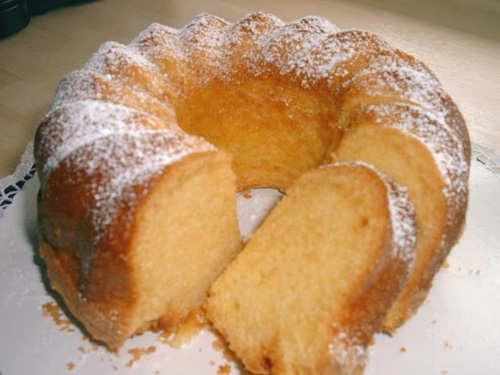
\includegraphics[width=.80\textwidth]{frames/img/eierlikoerkuchen}
        \end{center}
    \note{
        \begin{itemize}
            \item like it here
            \item learned a lot
            \item scope was too wide, lklfuse + utils would have been enough
            \item could have asked for help more often
            \item thank everyone who made me feel welcome, gave advice, talked Swedish with me even if it was a bit of a hassle
            \item learned to work in Sweden
        \end{itemize}
         }
    
    
    
\end{frame}


\begin{frame}

\frametitle{Backup Slides}
    
\note{note text}



\end{frame}


